\chapter{Outputs and results}
\label{cap:AIG:Outputs}
\begin{Resumen}

This first chapter aims on giving the reader a panoramic overview of the problematic of study, raising consciousness not only on the work carried out but on a more introspective PoV of its day-to-day approach, yet its working atmosphere. Thus, the \nameref{sec:Intro:thesis-purpose} is firstly stated, altogether with a \nameref{sec:intro:background} and a work-frame environment within \nameref{sec:Intro:HERGE}\footnote{Projet HERGE was the teamwork in which my \ingles{stage} was framed, will be explained in detail in the section \ref{sec:Intro:HERGE}} brief inductions, technically enriched on  \nameref{sec:intro:software} section.  

\end{Resumen}
\PartialToc
% ---------------------------------------------------------------------
% ---------------------------------------------------------------------


\bigskip
\lettrine[lines=2]{\textbf{S}}{}hall be kept in mind that the final objective of the undergone work was to end up with a logical, representative layout of the corporate electrical network in HV and super HV. In the following, several livrables of the work pursued will be presented, in order to shed more light on the validity of the work undergone, sustaining its methodology and approaching.

In addition, a path guide of the steps undergone to reach the final solution is performed, for the reader to more logically  understand the decisions taken, and the improvements introduced. 

\section{Overview}

In a first approach, the different element typologies have been represented gradually, by affecting them incrementally the iconographic properties for correctly retaken the UML structuring, plus the conventional properties following the \nameref{subsub:AIG:normative:elec-representation}.

In this way, the functional schemes will be step by step complemented with the introduction of every \textit{Class} notion.

Once the functional structure retaken in FME as explained in the \nameref{subsub:AIG:diagram-layout:object-picto- properties} subsection, position looped assessment in ArcGIS will modify the post positions gradually.

\section{Utilization}

Conversely, several objectives have been introduced following users expectancy, and therefore several applicability have been introduced on that point.

In a future extent, a gateway for managing the position of every element and adhere to each of them the pictographical properties as conceived in the actual interface, so that users are not impacted on the whole scheme display. Nonetheless, the complete hierarchical scheme will be automatically reproduced, so that every modification could be exploited to the totality of the diagram, making new posts aggregation much more logical and work-demanding.

\subsection{Users}

The most controversial point was the staticity of users, regarding Herge capabilities and features. Taht is, after been already used to a static, clear and functional (yet not optimal, as daily anomalies were identified) portal, users seemed skeptical to any change, and the complete automatizing of Herge's schemes will comport a major one.

Taking into account that most of on-field operations were traditionally performed on the basis of Herge schemes, the risk undertaken of a non-performing comprehension of a topology due to changing pictographs was substantially high.

\subsection{Industrialization process}

Firstly fed on RDF databases, exchanges with StanWay lead to the providing of structured XML files, deeply transformed through several databases feeding and metadating operations.

Several steps embarked the complete schema reproduction. Its different parts where systematically added, by following a continuous logic. Hence, each element kind was added at a pase, completing the schema systematically. The elements classification can be found in the section regarding \nameref{cap:AIG:diagram:FME} treatment.

It is therefore this treatement which have embarked the majority of evolution regarding industrialization. Its files occuping more than """ KB and their aspect as shown in the figure hereafter, their modularization in the lattest phases of ist implementation, plus the introduction of a GIT for version controlling has boosted its industrialization possibilities, yet as its clarity and retaking facility.

IMAGENES DEL TRATAMIENTO FME ANTES Y DESPUES DE LA MODULARIZACION

\subsubsection{HERGE V2}

At a second stage, and after a proper object projection and interconnection, its positionning was managed through ORACLE linked bases, who were using in the actual handmade diagram layout confection. ArcGIS toolkit enabled its projection on a Webplayer, as well as the elements position modificiation. 

Images of the diagram layout aspect before and after the implementation of the intelligent algorithm can be found hereafter.

IMAGEN DE ANTES Y DESPUES DE UTILIZAR EL NETWORK ANALYST DE ARCGIS


% -------------------------------------
\begin{figure}[h!]
	\bigskip
	\begin{center}
		\parbox{.45\textwidth}{%
		\href{https://polimedia.upv.es/visor/?id=c73f835e-9387-7643-9473-335796a00932}
			{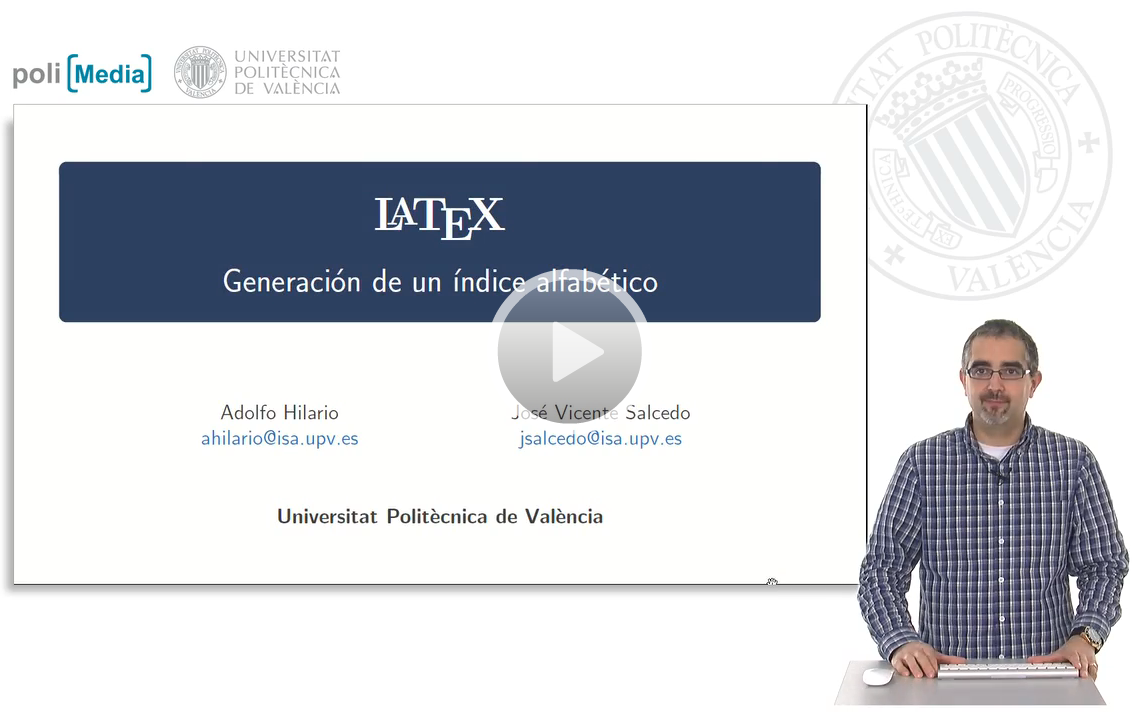
\includegraphics[width = .45\textwidth]{0.figuras/poliMedia_makeindex.png}}}\hfill
		\parbox[t]{.45\textwidth}{\caption{Veo poliMedia: ``Generaci de un ndice alfabico''.
			Haz clic sobre la imagen para acceder al vdeo}
			\label{fig:makeindex}} 
	\end{center}
\end{figure}
\section{Improvement lines}

HABLAR CON HENG ASI COMO CON GERMAN PARA PODER METER TODO ESTO EN COHERENCIA CON LAS MODIFICAICIONES QUE ESTAN HACIENDO AHORA MISMO 

\section{Constraints}

VER LAS REPERCUSIONES QUE EL SEGUIR UTILIZANDO LA BASE DE AUTOCAD PODRIA TENER EN EL FUTURO DESARROLLO DEL PROGRAMA

\subsubsection{Technical constraints}
\subsubsection{Financial constraints}
\subsubsection{Time constraints}
\subsubsection{Usage constraints}
